This section explains and shows the final design of the application. The final design is a result of all the design analysis done in previous chapter\todo{Skal det stå der? Skal have en form for intro} 

\begin{figure}[H]
\begin{minipage}[t]{0.5\columnwidth}
\centering
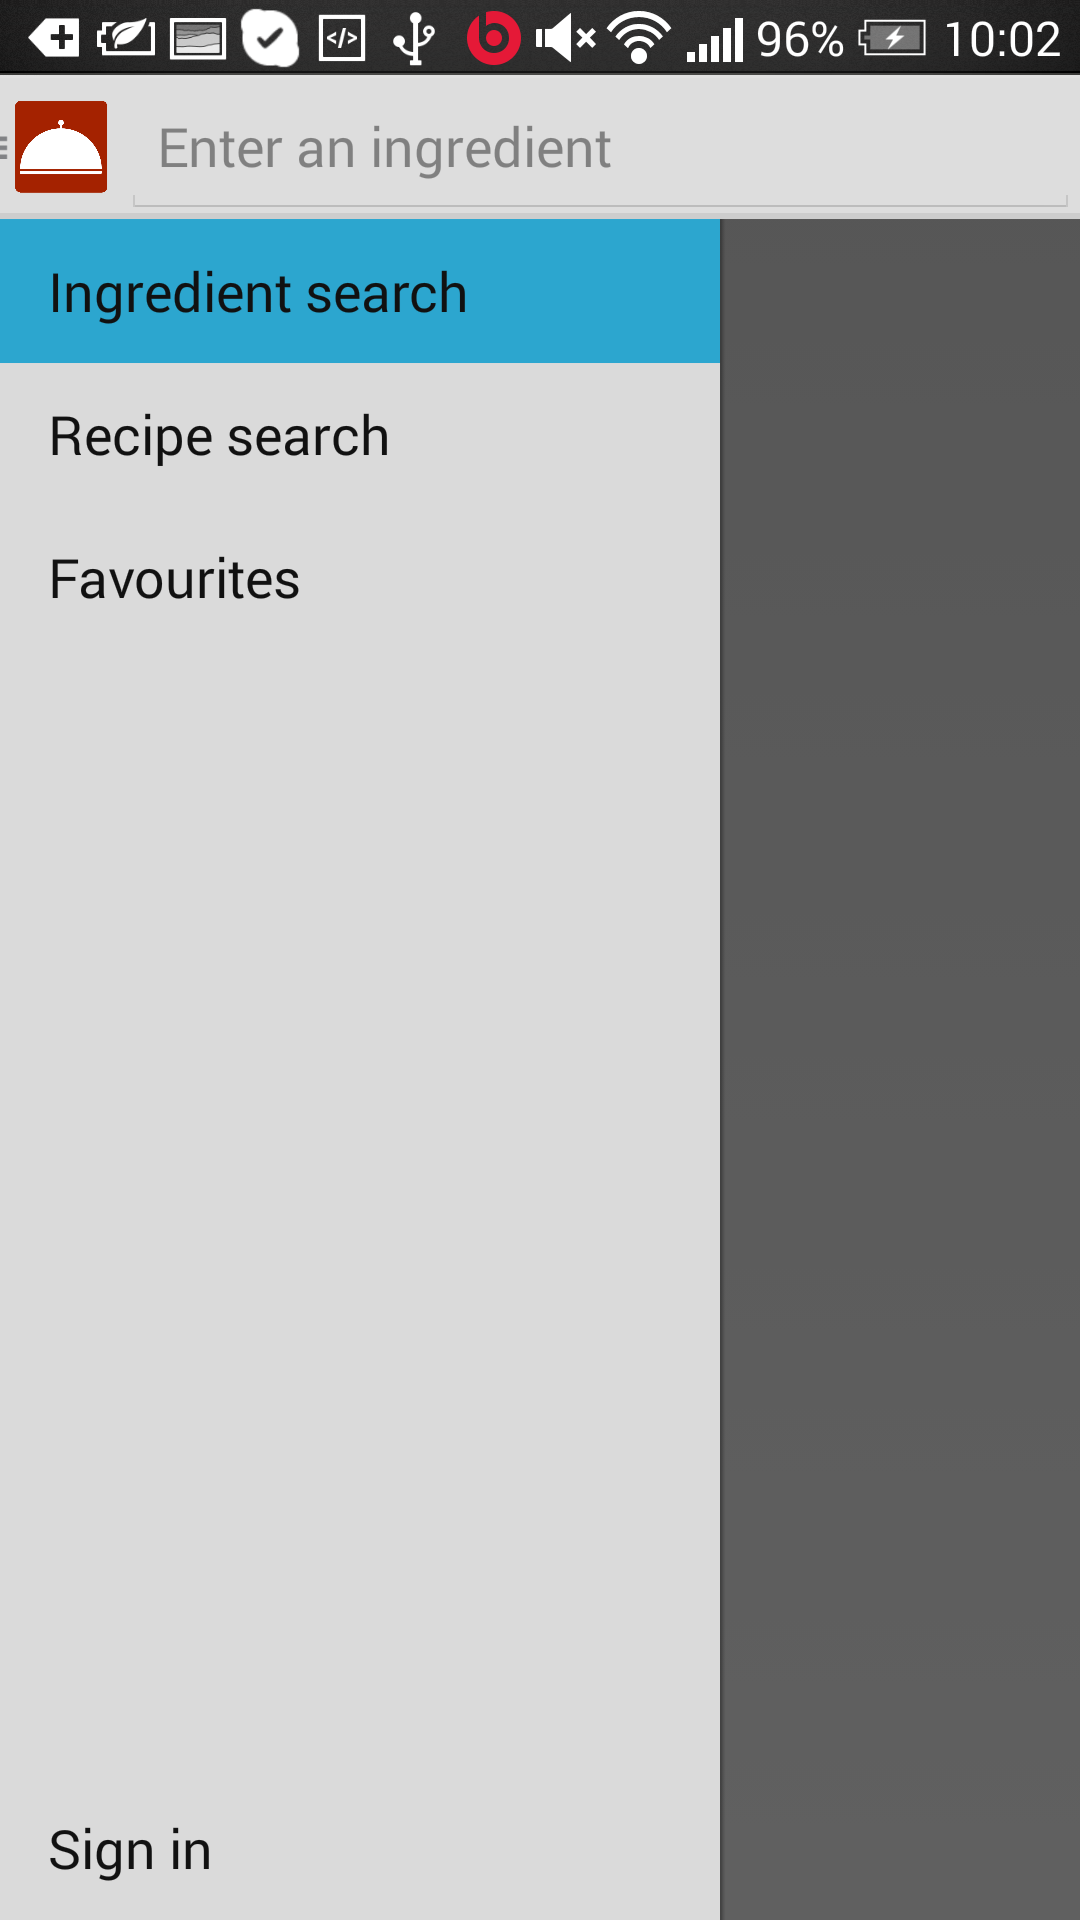
\includegraphics[width=0.7\columnwidth]{img/screenshots/finaldrawer.png}
\caption{Navigation drawer\label{fig:navdrawer1}}
\end{minipage}
\hspace{0.5cm}
\begin{minipage}[t]{0.5\columnwidth}
\centering
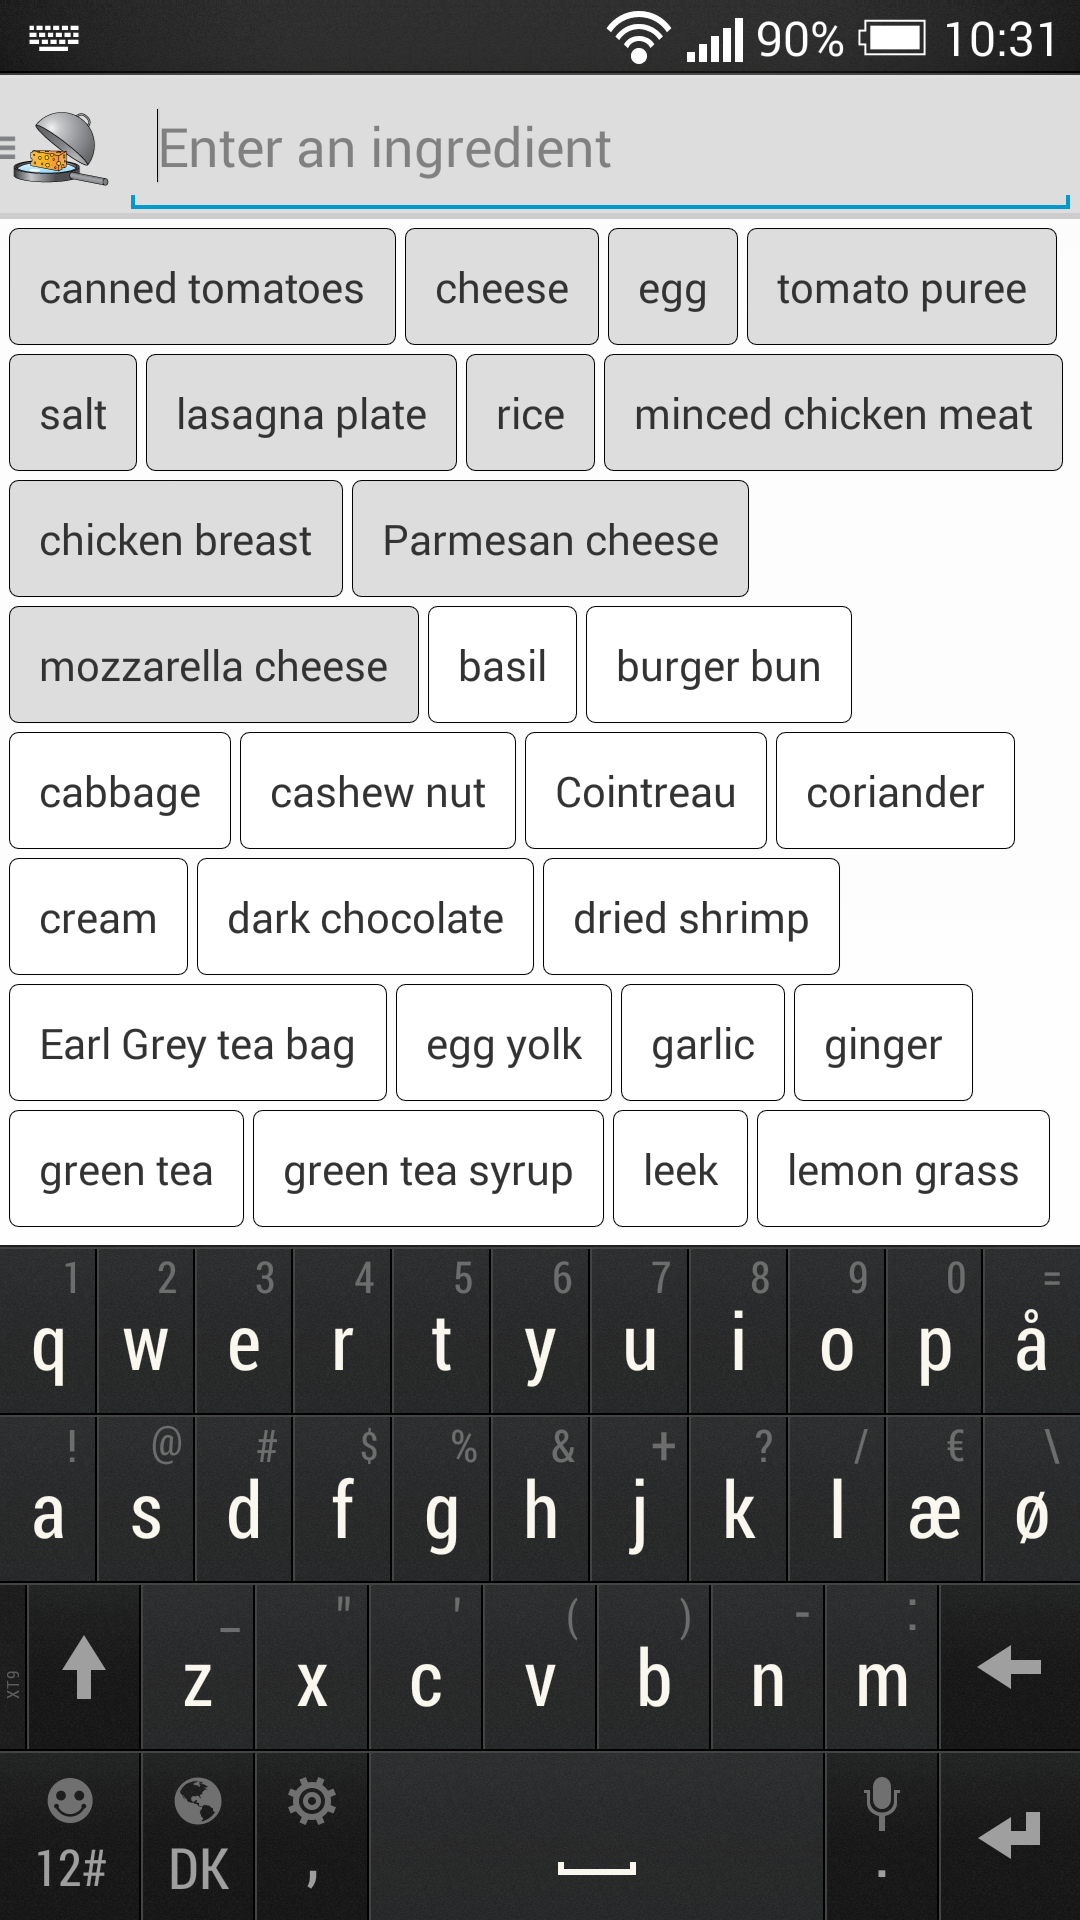
\includegraphics[width=0.7\columnwidth]{img/screenshots/finalwordcloud.png}
\caption{Word cloud\label{fig:wordcloud}}
\end{minipage}
\end{figure}

The first time the user opens up the application they are prompted with a navigation drawer, as seen on \autoref{fig:navdrawer1}. The reason this is shown the first time the application is opened is to inform the user that it is available, as this is the tool they will be using to navigate between the different pages in the application. The navigation drawer is available from every page of the application. The navigation drawer is an overlay of the application content but not the action bar\citep{guidelines-navigationdrawer}.

The user opens the navigation drawer either by swiping from the left edge of the screen or by clicking the icon in the top left corner and it is closed either by clicking outside of the navigation drawer, by clicking the icon in the top right corner again, by swiping from right to left anywhere on the screen, or by pressing back.

If the user closes the navigation drawer and presses the search field on the action bar where it says ``Enter an ingredient'', the word cloud pops up. The word cloud is preloaded with suggestions for ingredients that can easily be clicked and added to the search. The user is also able to search for ingredients by typing in the name. When the user types, a list of suggestions will come up and the user can either press a suggestion from the list or press enter and add the first ingredient in the suggestion list to the search. The details of the search suggestions are explained later.

\autoref{fig:wordcloud} shows the word cloud with a number of ingredients added. The grey labels are included in the search, whereas the white labels are only suggestions the user can press and are not included in the search.

\begin{figure}[H]
\begin{minipage}[t]{0.5\columnwidth}
\centering
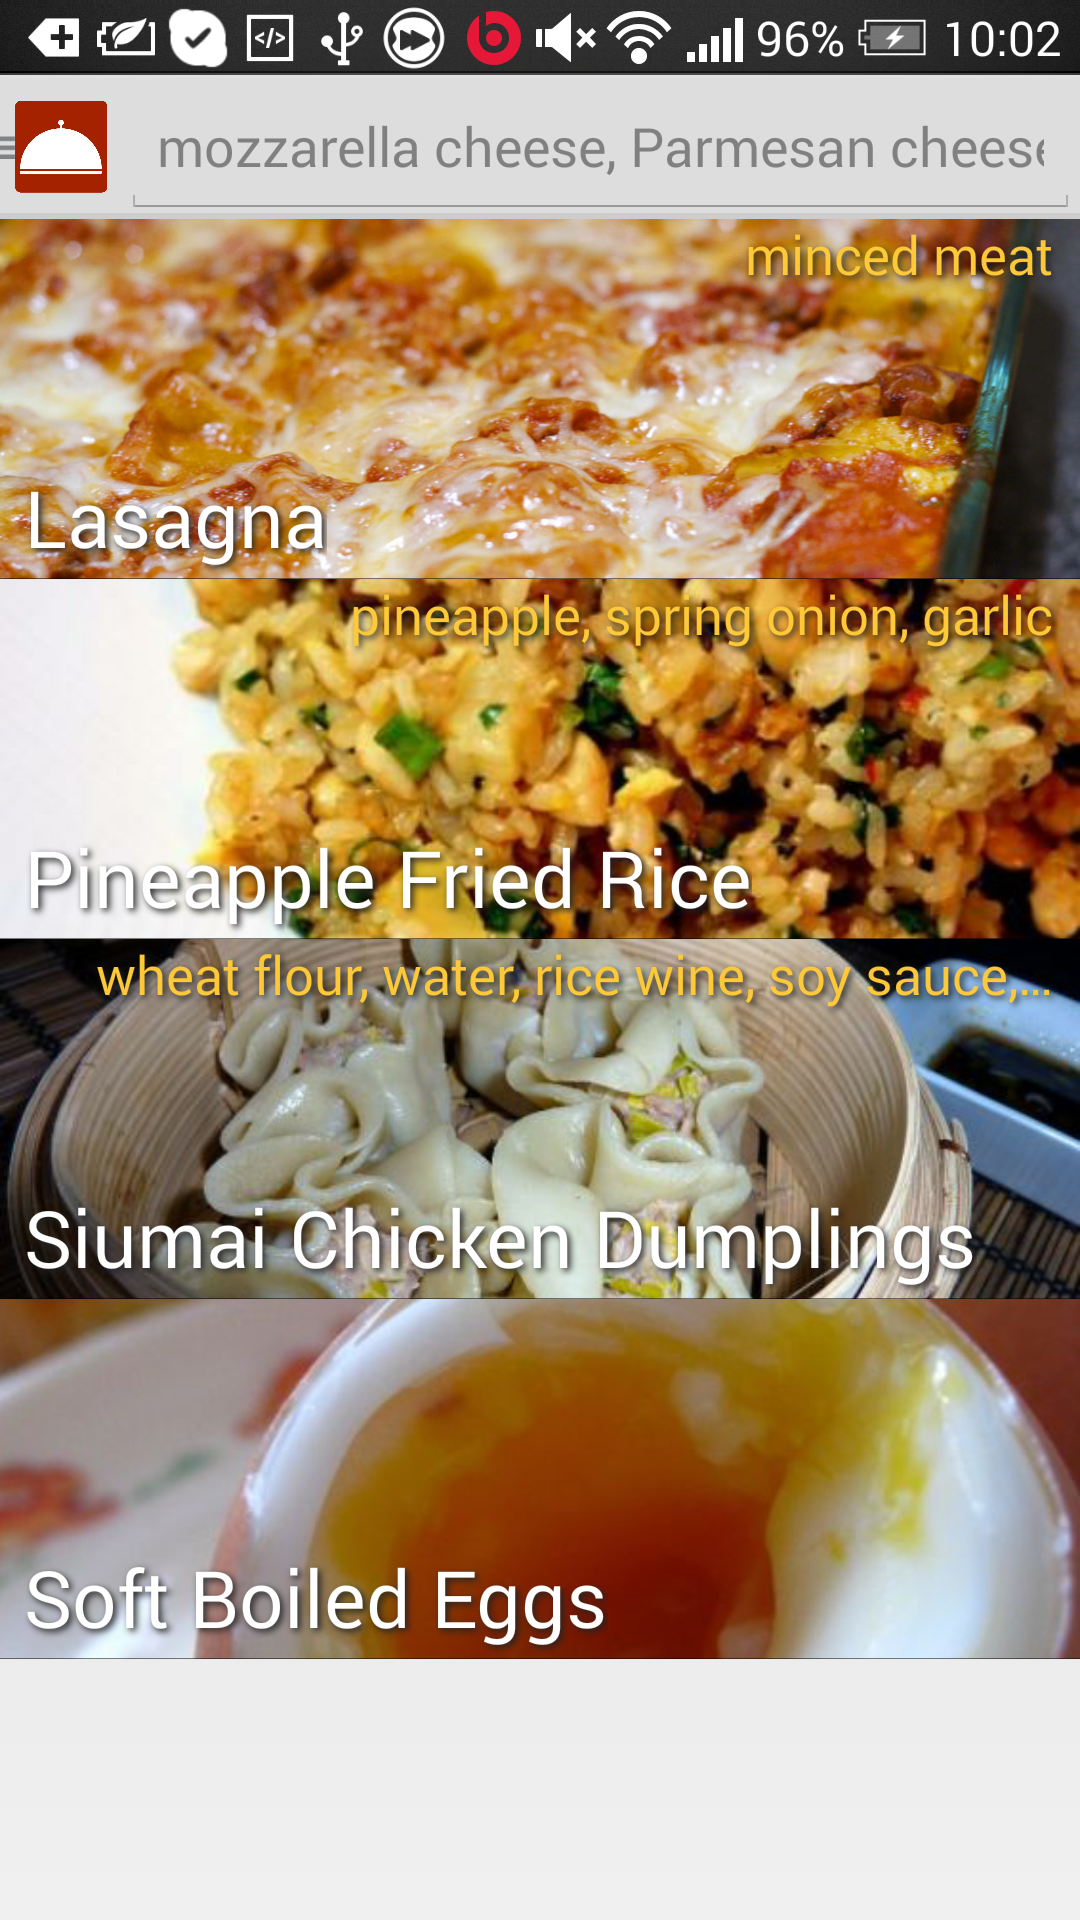
\includegraphics[width=0.7\columnwidth]{img/screenshots/finallist.png}
\caption{List of recipes\label{fig:recipelist}}
\end{minipage}
\hspace{0.5cm}
\begin{minipage}[t]{0.5\columnwidth}
\centering
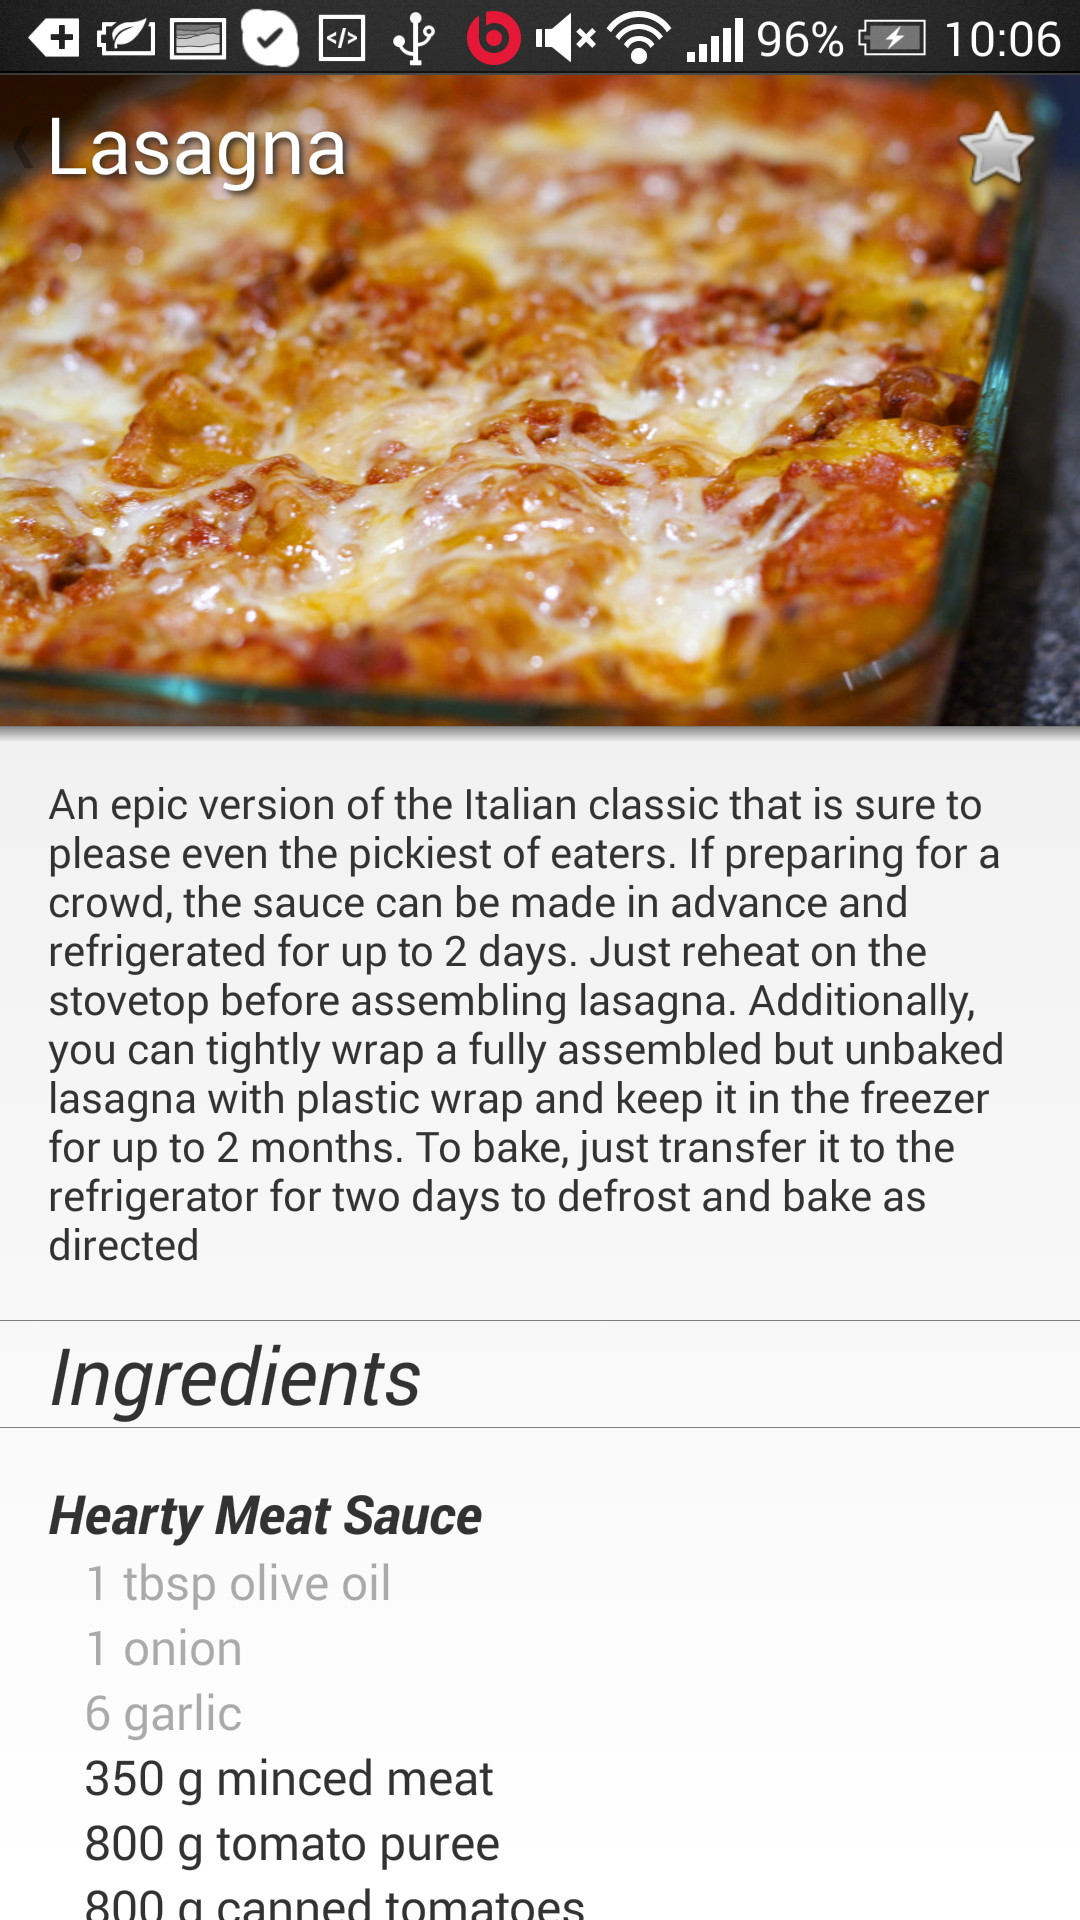
\includegraphics[width=0.7\columnwidth]{img/screenshots/finalrecipe1.png}
\caption{Recipe layout\label{fig:recipe1}}
\end{minipage}
\end{figure}

\begin{figure}[H]
\begin{minipage}[t]{0.5\columnwidth}
\centering
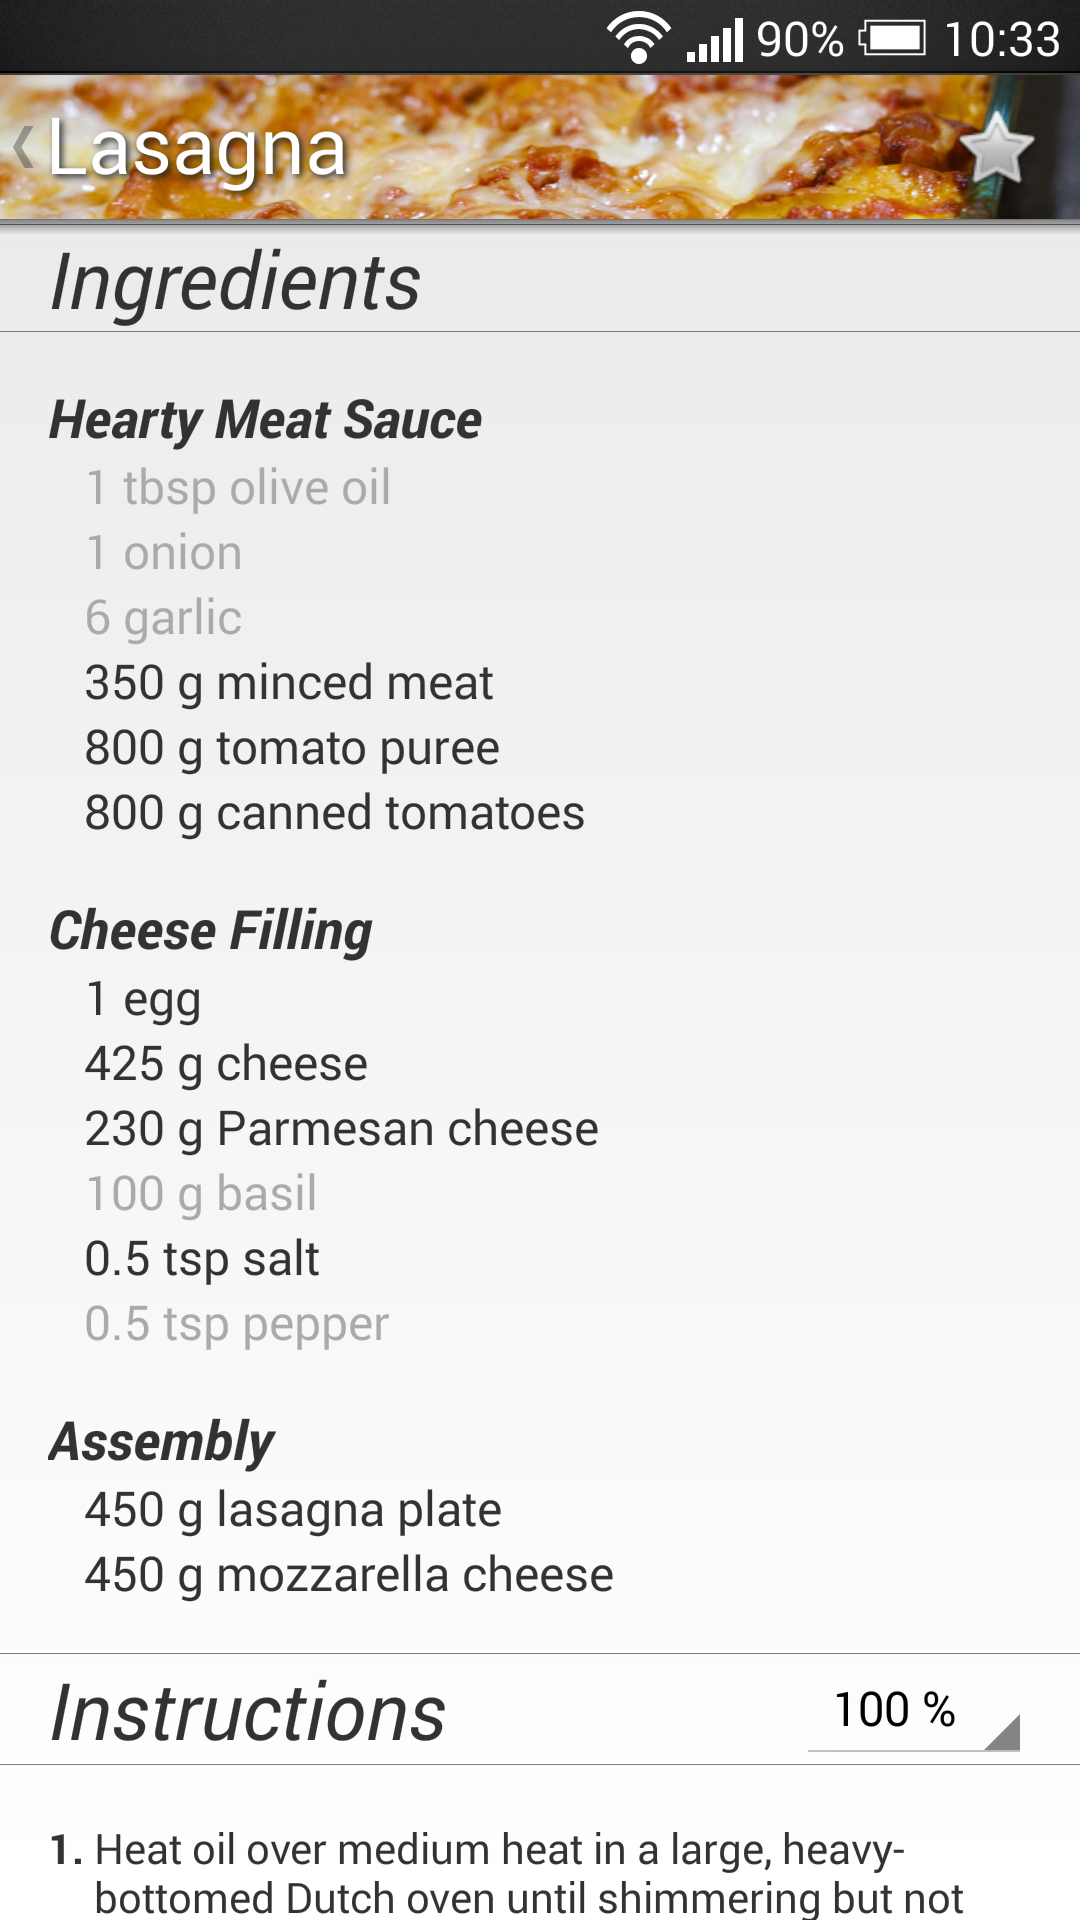
\includegraphics[width=0.7\columnwidth]{img/screenshots/finalrecipe2.png}
\caption{Recipe layout\label{fig:recipe2}}
\end{minipage}
\hspace{0.5cm}
\begin{minipage}[t]{0.5\columnwidth}
\centering
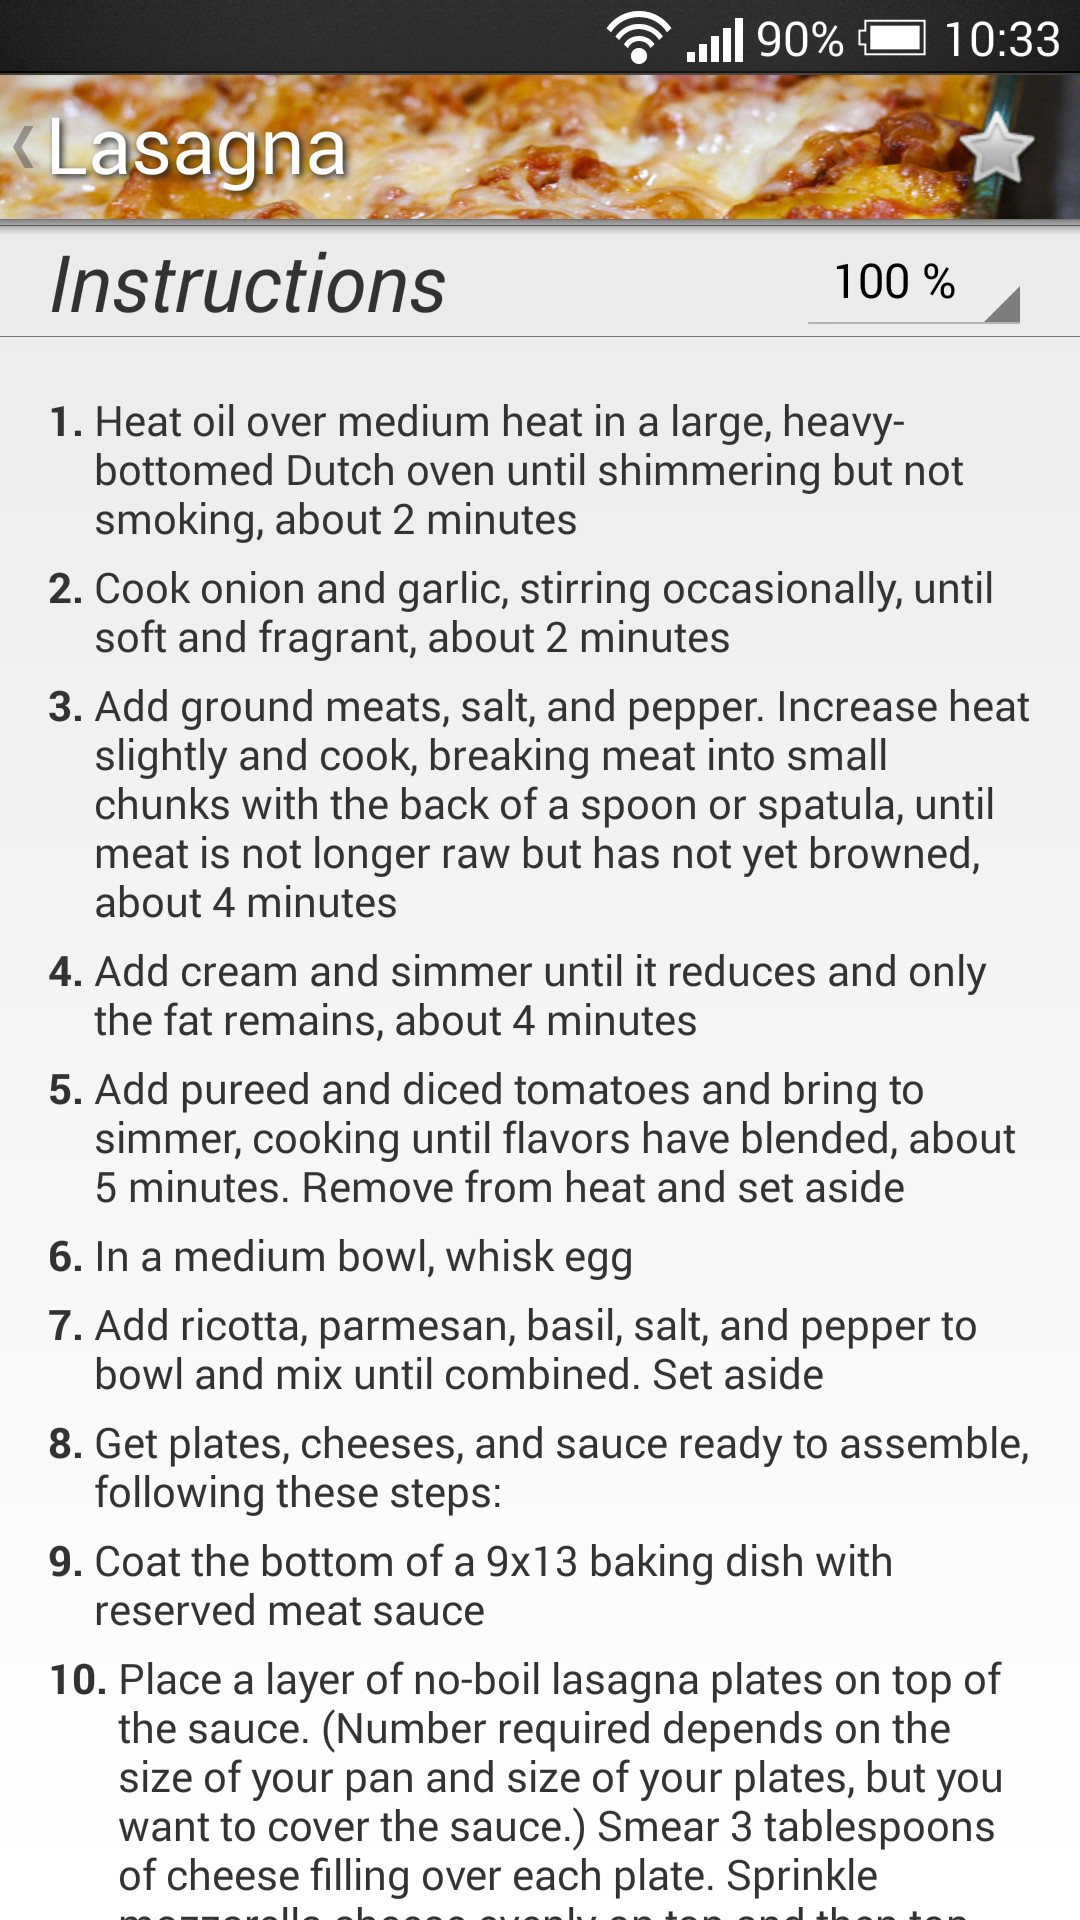
\includegraphics[width=0.7\columnwidth]{img/screenshots/finalrecipe3.png}
\caption{Recipe layout\label{fig:recipe3}}
\end{minipage}
\end{figure}


If the user presses the hardware back button or presses the enter key without having input anything into the search field, a search is performed. \autoref{fig:recipelist} shows the list of recipes based on the ingredients entered in \autoref{fig:wordcloud}. The search field has always changed its text, it now shows a some of the ingredients that the user has included in the search, the search field itself works like before. If the ingredient search exceeds the number of recipes that can be shown on the screen, they will automatically be downloaded as the user scrolls down. This also applies to the list of recipes in recipe search and in favourites.


The yellow text on some of the recipes indicates what ingredients the user is missing in order to have all mandatory ingredients for the recipe.

If the user presses a recipe it will open and they will see the full recipe. This can be seen on \autoref{fig:recipe1}, \autoref{fig:recipe2}, and \autoref{fig:recipe3}. The three figures shows an example of a full recipe. The grey ingredients are optional, where as the black ingredients are mandatory. 


\autoref{fig:recipe2} shows the list of ingredients needed to make the recipe, listed in groups. \autoref{fig:recipe3} shows the instructions in order to make the recipe, the user is able to change the font size in the top right corner. The user is also able to favourite a recipe by pressing the star in the top right corner. In order to favourite a recipe the user needs to be signed in.

\begin{figure}[H]
\begin{minipage}[t]{0.5\columnwidth}
\centering
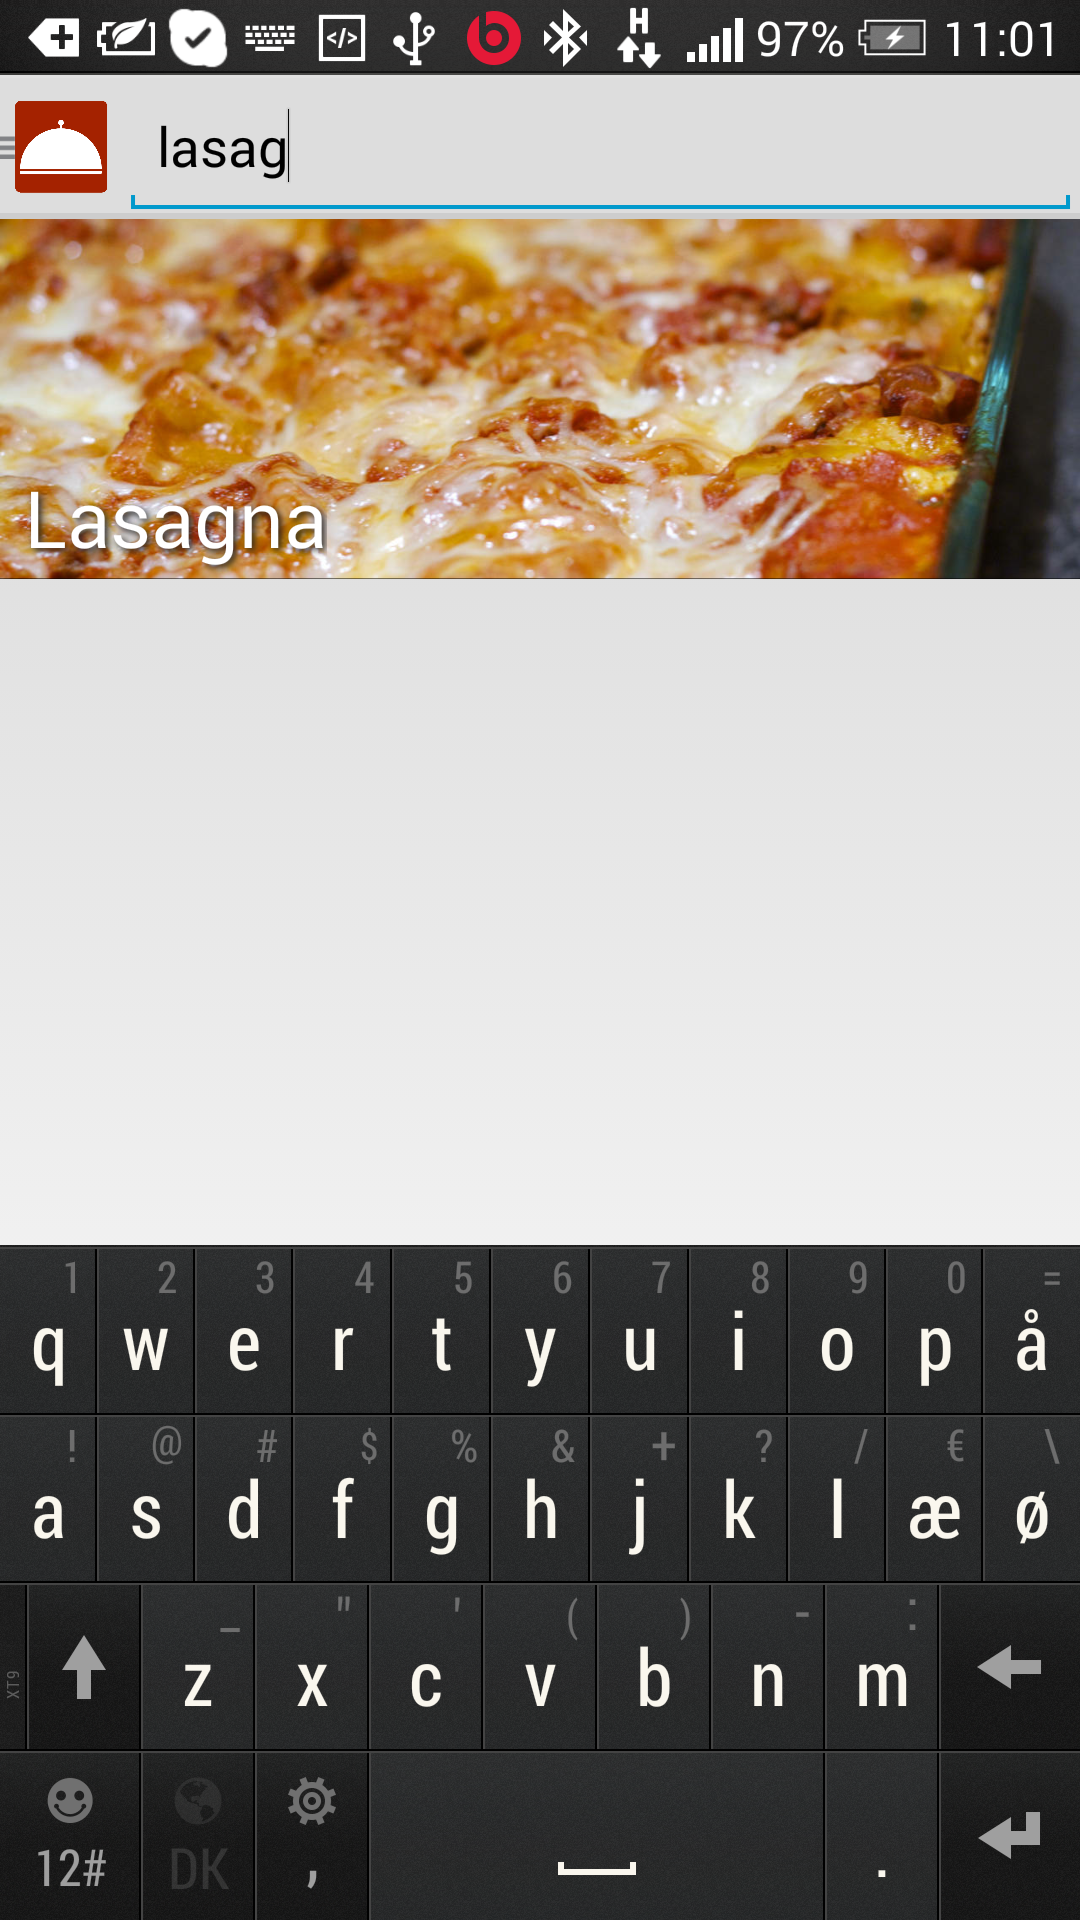
\includegraphics[width=0.7\columnwidth]{img/screenshots/finalrecipesearch.png}
\caption{Recipe search\label{fig:recipesearch}}
\end{minipage}
\hspace{0.5cm}
\begin{minipage}[t]{0.5\columnwidth}
\centering
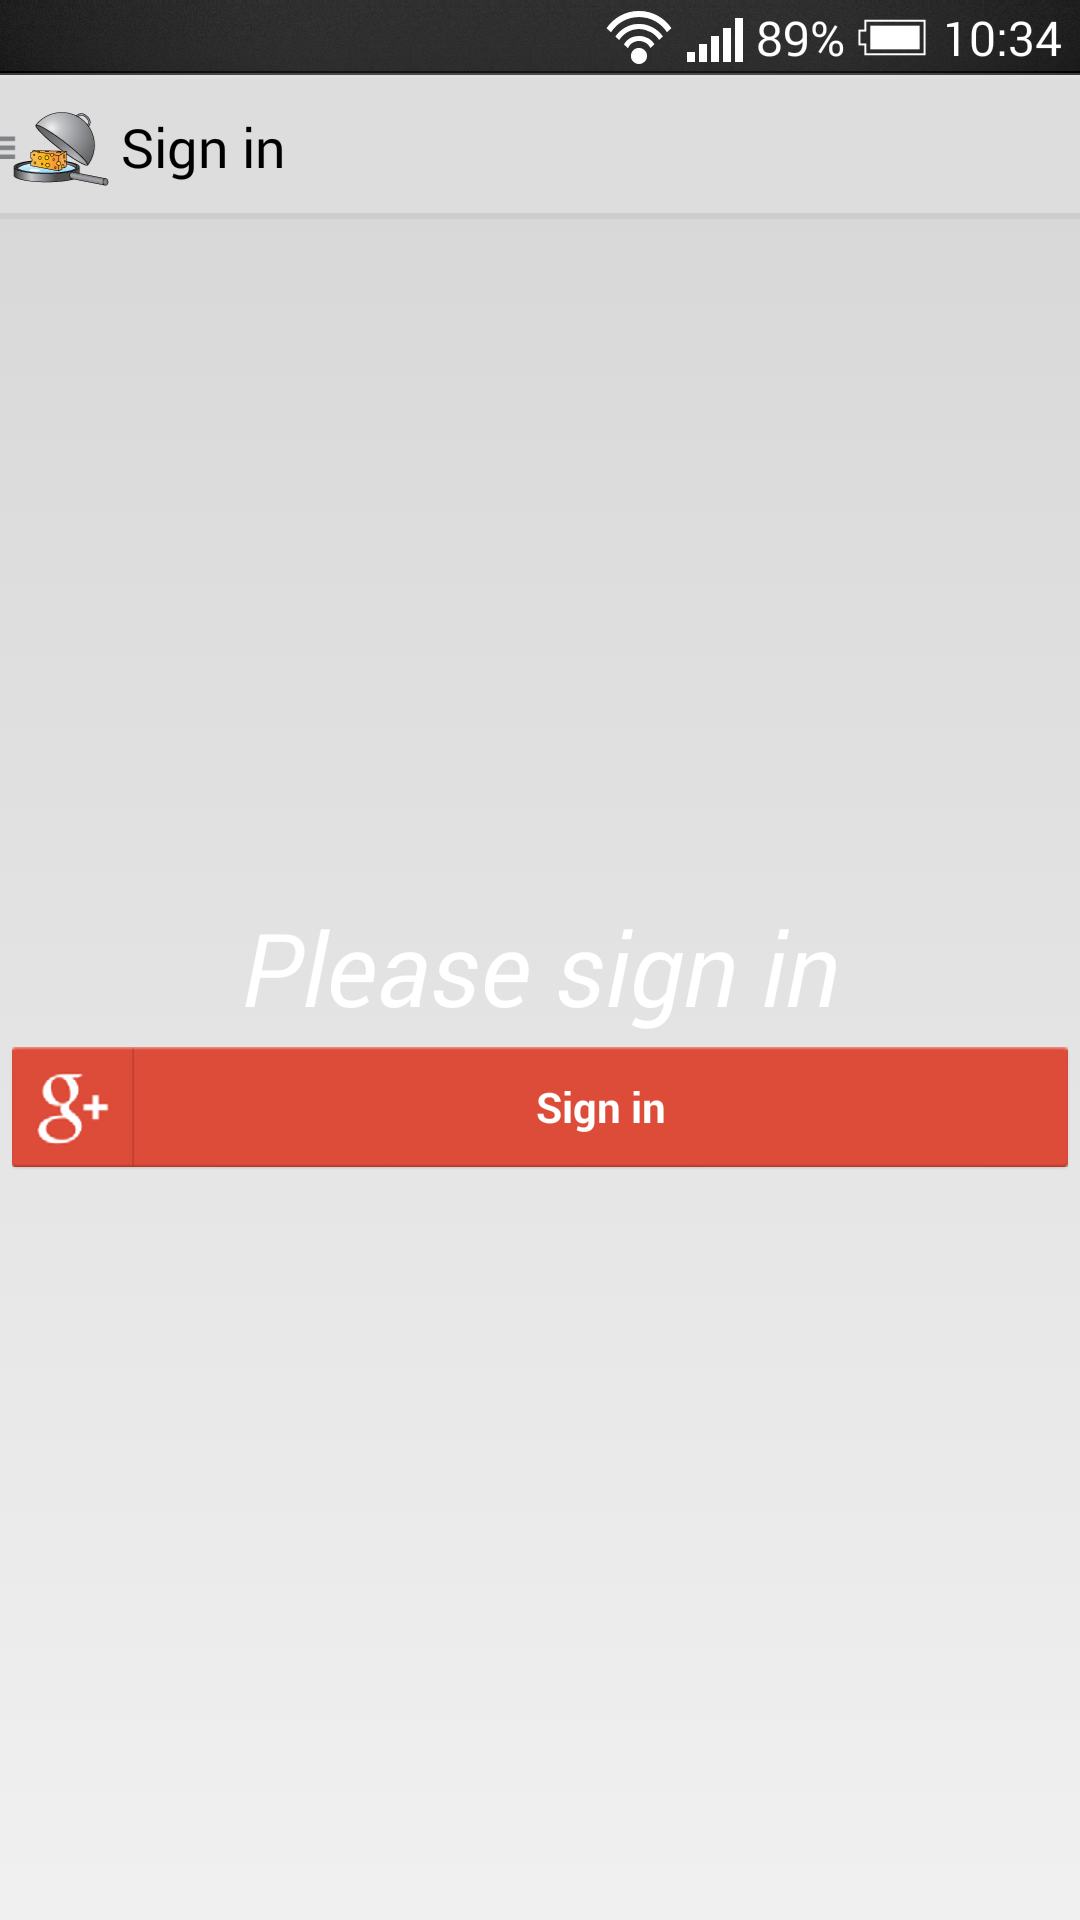
\includegraphics[width=0.7\columnwidth]{img/screenshots/finalsignin.png}
\caption{Sign in\label{fig:signin}}
\end{minipage}
\end{figure}

The user is not just limited to searching for recipes based on ingredients, they can also search for recipes using free text, this is shown in \autoref{fig:recipesearch}. This allows the user to search for a recipe based on its name or words included in the recipe description. 

When a user wants to access their favourites, they have to be signed in, incase the user tries to access their favourite recipes without being signed in, they are asked to log in using Google+, this is shown in \autoref{fig:signin}.

\begin{figure}[H]
\begin{minipage}[t]{0.5\columnwidth}
\centering
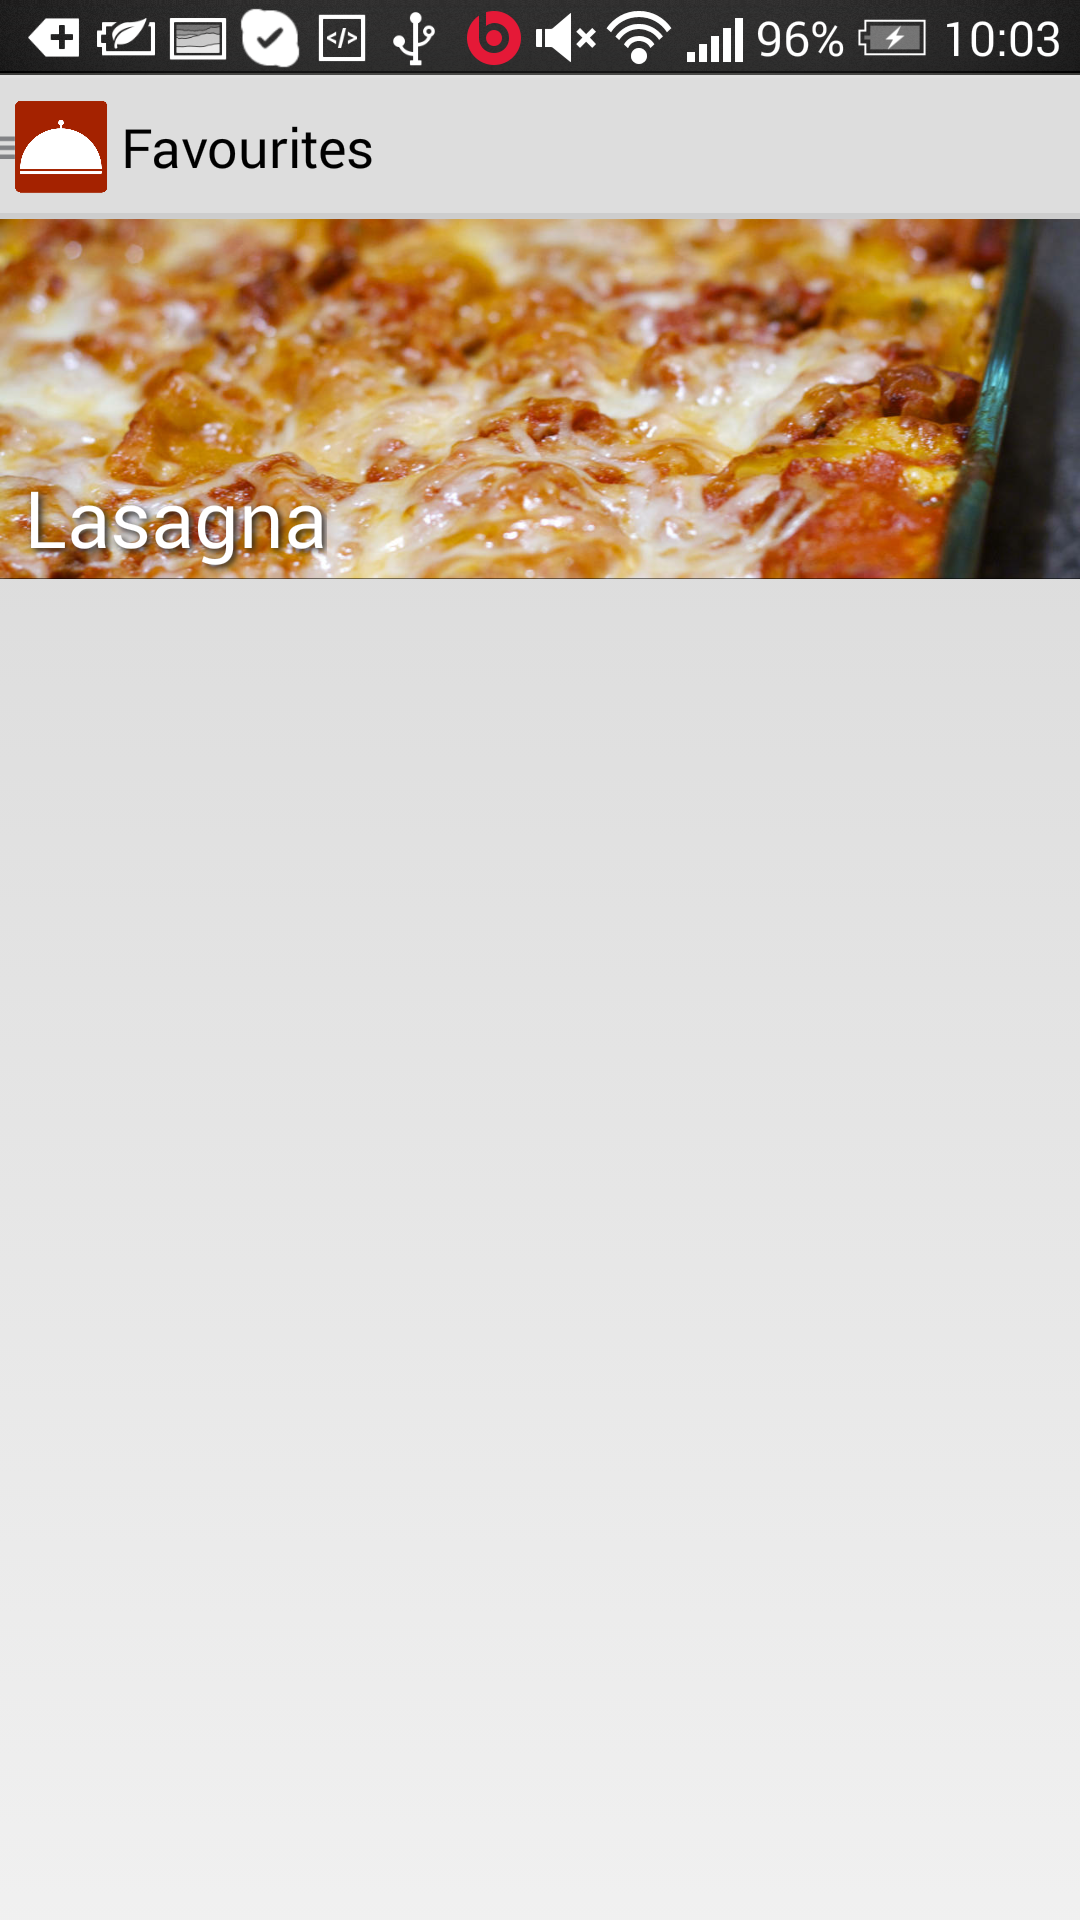
\includegraphics[width=0.7\columnwidth]{img/screenshots/finalfavourite.png}
\caption{Favourite list\label{fig:favourite}}
\end{minipage}
\end{figure}

 After the user has logged in, they are able to access their favourite recipes as shown in \autoref{fig:favourite}. The user is able to click the recipes and open the full recipe. In order to remove recipes from favourites, the user can either long click or open the recipe and press the star again.